\documentclass{article}
\usepackage{graphicx}
\usepackage{float}
\usepackage{caption}
\begin{document}

\title{GC Content in Yeast}
\author{Bo\v{z}ena Nevinskien\.{e}}
\maketitle

\section{About the study}
\emph{Saccharomyces cerevisiae} is a single-celled eukaryote that is frequently used in scientific research. It is an attractive and very popular model organism due to the fact that its genetics are easily manipulated, and it is very easy to maintain in the lab. 
This single-celled organism is also important in industry, where it is used to make bread, beer, wine, enzymes, and pharmaceuticals. The \emph{Saccharomyces cerevisiae} genome is approximately 12 Mb, organized in 16 chromosomes.


According to the genome databases, GC content of \emph{Saccharomyces cerevisiae} is 38.3\%. 
The goal of this study is to check if it is true. 
Also to determine if all yeast genes have the same GC content, and if not, why? 
GC content is very important in experiments, such as PCR, where GC content is important for primer designing, predicting their annealing temperature. Also, GC content showed a quadratic relationship with genome size, with the decreases in GC content in larger genomes possibly being a consequence of the higher biochemical costs of GC base synthesis.

For this study we randomly selected 3 strains or yeast and found their possible open reading frames:
\begin{enumerate}
	\item EC9-8: found 8622 possible open reading frames.
	\item VL3: found 9859 possible open reading frames.
	\item YS9: found 8341 possible open reading frames.
\end{enumerate}

In this study, we did not search for reverse complement open reading frames on the antisense DNA chain.                    
Also, not all reading frames may be accurate. The only criteria, that we followed is that the open reading frame must be
at least 50 codons in length between start codon (ATG) and stop codons (TAA, TAG and TGA).
After finding these ORFS, we calculated GC ratio in each of the ORFS and analysed frequency of GC ratios.

\subsection{EC9-8 results}

\begin{minipage}{0.5\textwidth}
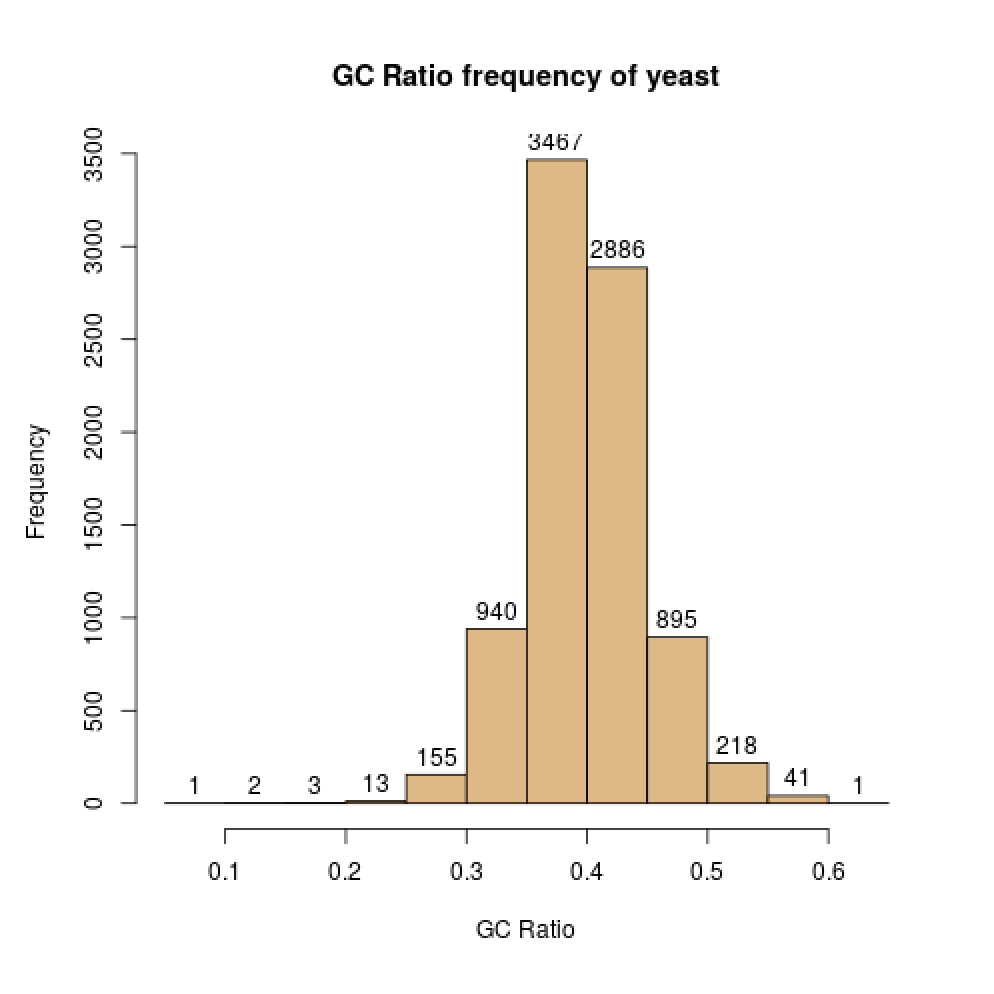
\includegraphics[width=\textwidth]{images/EC9-8_ASinica_2011_AGSJ01000000.eps}
\captionof{figure}{GC ratios of EC9-8}
\end{minipage}
\begin{minipage}{0.5\textwidth}
EC9-8 is a haploid cadmium-resistant derivative of a yeast isolated from the valley bottom of Evolution Canyon 
at Lower Nahal Oren, Israel. This yeast strain had the highest number of outliers in GC ratio.
But on the average of G and C nucleotides in EC9-8 yeast strain's possible ORFS was approximately 39.94\%. More than 70\% of ORFS had the G and C ratio between 35\% and 45\% (Fig. 1). \vspace{1cm}\\
\end{minipage}


\subsection{VL3 results} 

\begin{minipage}{0.5\textwidth}
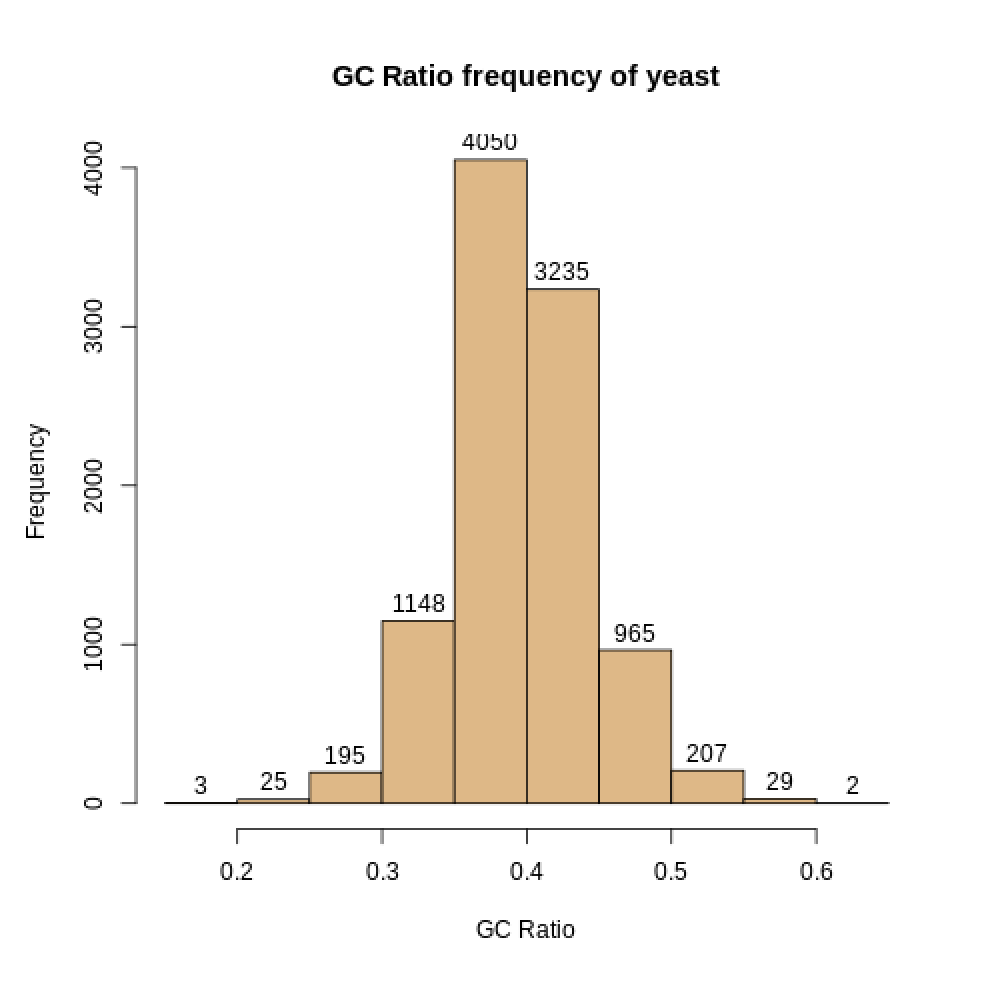
\includegraphics[width=\textwidth]{images/VL3_AWRI_2011_AEJS01000000.eps}
\captionof{figure}{GC ratios of VL3}
\end{minipage}
\begin{minipage}{0.5\textwidth}
VL3 was isolated in Bordeaux, France, and is most suited to the production of premium aromatic 
white wines with high thiol content (citrus and tropical fruit characters). 
VL3 has a whole-chromosome amplification of chromosome VIII, as well as 54 ORFs that are missing in other strains.
The average of G and C nucleotides in VL3 yeast strain's possible ORFS was approximately 39.67\%
(Fig. 2).  
\vspace{1cm}\\
\end{minipage}

\subsection{YS9 results}


\begin{minipage}{0.5\textwidth}
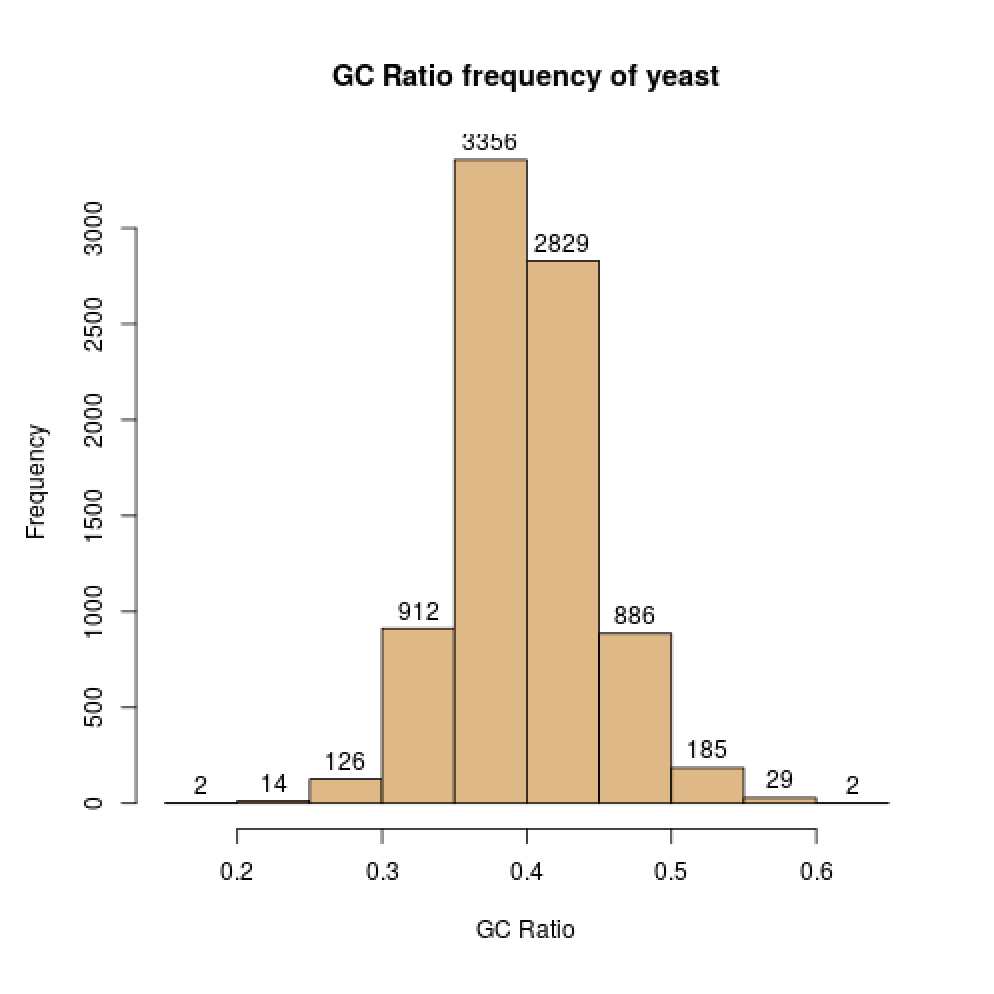
\includegraphics[width=\textwidth]{images/YS9_Stanford_2014_JRIB00000000.eps}
\captionof{figure}{GC ratios of YS9}
\end{minipage}
\begin{minipage}{0.5\textwidth}
YS9 is one of the Singapore's baking yeast strains.
The average of G and C nucleotides' ratio in EC9-8 yeast strain's possible ORFS was approximately 39.97\% (Fig. 3). 
\vspace{1cm}\\
\end{minipage}

\section{Conclusions}


\begin{minipage}{0.5\textwidth}
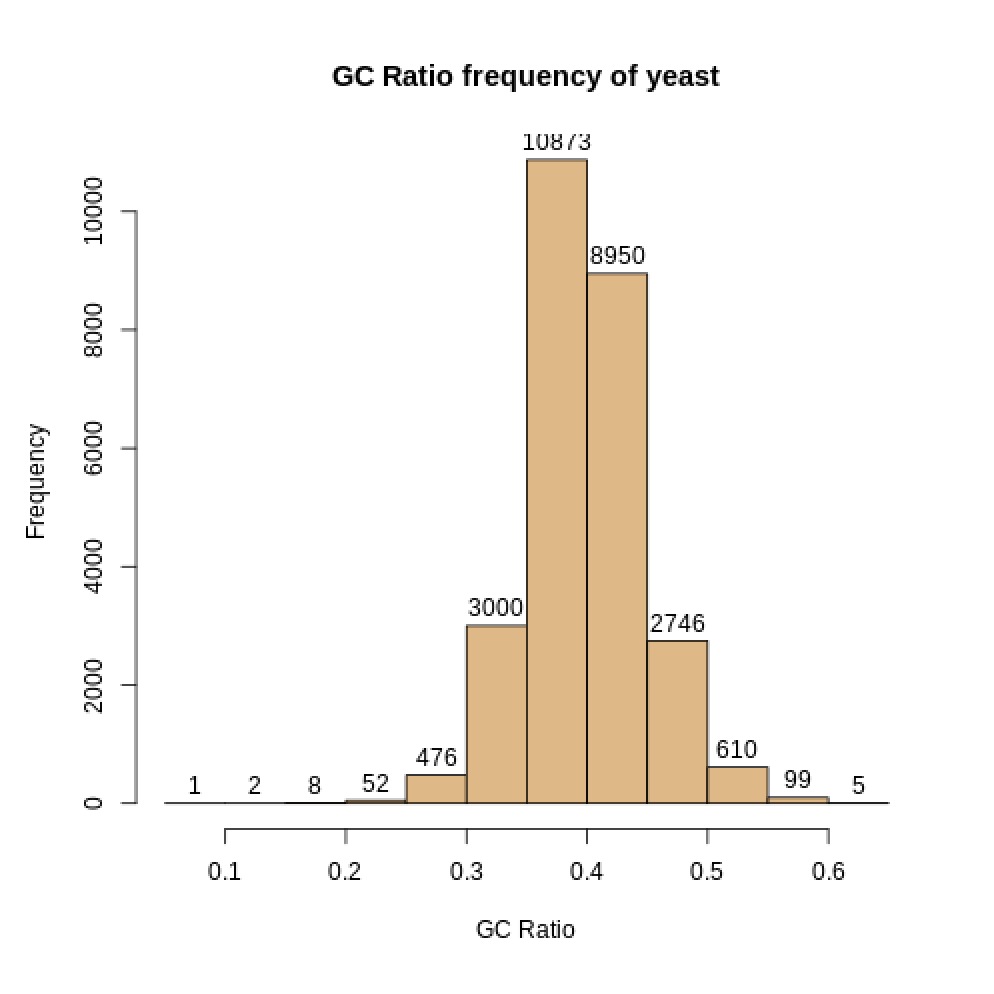
\includegraphics[width=\textwidth]{images/AllGenomes.eps}
\captionof{figure}{GC ratios of all three strains}
\end{minipage}
\begin{minipage}{0.5\textwidth}
Overall in all 3 strains the mean of G and C nucleotides was about 39.86\% of all nucleotides (Fig. 4). 
According to Anderson-Darling normality test, none of the GC ratio results were distributed normally. Although, we have a large sample size, so we can compare GC ratios between 3 strains with a T test. Results have shown, that GC ratios of strains YS9 and 
EC9-8 are not significantly different. But both of those strains' GC ratio means significantly differ from VL3 strain's.
\vspace{1cm}\\

\end{minipage}

\bigskip
All in all, the most possible open reading frames had GC ratios between 0.35 and 0.45. The GC-content of all three strains was similar, but not perfectly 38.3\% as it was predicted. This 1.56\% difference seems very small but it is significant. In the future studies we should consider inculing reverse complement open reading frames for more accurate results.

\end{document}
